\chapter{Parser}

\emph{\textbf{Autoren:} David Schneller, Dominik Kreutzer}

Das Parser-Modul liest den gegebenen Assembler-Code, führt alle gegebenen
Compiler-Direktiven aus und generiert für jedes Argument einen Syntax-Baum, der
an die Architektur übergeben wird.  Außerdem reserviert er den über die
Reservierungs- und Definierungsdirektiven festgelegten Speicher.

Somit entspricht der Parser dem Assemblierer.  Die Trennung von Architektur und
Parser wurde vorgenommen, um Code-Duplikation zu vermeiden, die bei
Architekturen mit mehreren Dialekten auftreten könnten (bei X86 z.B. AT\&T- und
Intel-Syntax).

Weiterhin assistiert der Parser mit dem Befehlssatz der Architektur der GUI beim
Syntax-Highlighting und stellt syntaktische Fehler sowie nicht vorhandene Befehle fest.

\section{Ausführungsmodi}

Generell soll der Parser zwei Ausführungsmodi unterstützen:
\begin{itemize}
\item \textbf{Compile}: Kompiliert den kompletten Assemblertext und erstellt Symboltabellen und Syntaxbäume, reserviert Speicher und produziert Maschinencode.
\item \textbf{Update}: Betrachtet nur die Veränderungen zum vorherigen Assemblertext und aktualisiert Symboltabelle, Syntaxbäume entsprechend. Speicherreservierungsbefehle werden ignoriert.
\end{itemize}

\textbf{Compile} soll den Assemblertext in einen ausführbaren Zustand bringen. \textbf{Update} hingegen aktualisiert die interne Darstellung, falls während der Programmausführung der Quelltext verändert wird.

\section{Umsetzung (Referenzmodul)}

Das Referenzmodul, welches im Rahmen dieses Großpraktikums konstruiert werden
soll, wird als bekannter 2-Pass-Assembler realisiert. Wie die Architektur wird
dieses vorerst auf RISC-V (und hier einen bestimmten Dialekt) ausgelegt und
spezialisiert sein.

\subsection{1. Durchlauf}

Im ersten Schritt wird der rohe Assemblertext gelesen und in Zeilenbereiche
unterteilt, die jeweils einen Befehl mit allen zugehörigen Marken beinhalten.
Wenn wir im \textbf{Update}-Modus sind, betrachten wir hiervon nur die Befehle, die sich seit der letzten Ausführung geändert haben.
Diese Befehle werden anschließend in Objekte umgewandelt, wobei auch das Zeilenintervall und Datei des Auftretens gespeichert werden. Wir unterscheiden bei den Befehlen zwischen Direktiven und Operationen, bei ersteren differenzieren wir besonders. Alle Labels und auch Konstantennamen, die wie Labels behandelt werden, werden in die Symboltabelle mit ihrem
korrespondierenden (Text-)Wert geschrieben bzw. aktualisiert. Falls im \textbf{Compile}-Modus ausgeführt wird, wird die Symboltabelle zuvor noch geleert. Ebenfalls wird in diesem Modus der Speicher reserviert
und die Positionen der Daten berechnet, sowie die Befehlspositionen berechnet. Im \textbf{Update}-Modus erfolgt dies entsprechend nicht, die zugehörigen Direktiven werden einfach ignoriert.  Bei allen Makros wird Anfang und Ende erfasst und diese in eine separate Makroliste eingetragen.

\subsection{2. Durchlauf}

Wir haben nun eine Befehlsfolge von Objekten. In diesem Schritt werden nun die
Direktiven ausgeführt und die Labels mit ihrem Wert eingesetzt. Ein Befehl wird
zu einem Syntaxbaum umgewandelt. Im \textbf{Update}-Modus erfolgt dies nur für die Befehle, die geändert wurden oder von einem modifizierten Symbol abhängen. Zu diesem Zweck soll die Symboltabelle alle Befehlsreferenzen auf ein Symbol halten, sodass eine Suche nach abhängigen Befehlen schnell möglich ist.
Wegen möglichen unbekannten Datentypen anderer ISAs usw. stellt das Architektur-Modul hier eine Factory für
Knoten bereit.  Als Ausgabe dient schließlich eine
Liste von Befehls-Syntaxbäumen \emph{ohne} jegliche Direktiven. Diese wird dann dem Core zur Verfügung gestellt.

\begin{figure}[h!]
  \centering
  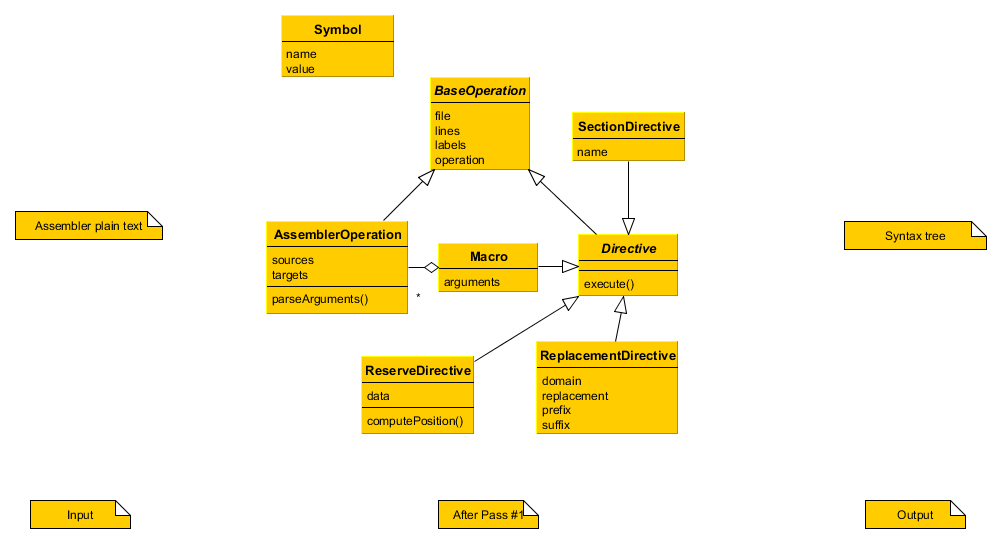
\includegraphics[width=0.8\textwidth]{../parser/figures/process.png}
  \caption{Eine grobe Skizze des geplanten Parsing-Prozesses nach aktuellem Stand.}
\end{figure}

\subsection{Geplante Unterstützung}
\subsubsection{Direktiven}
Unterstützt werden sollen:

\begin{itemize}
\item Makros
\item Speicherreservierungs- und Speicherbelegungs-Direktiven (z.B. resb, dd)
\item Konstantendefinitionen und Aliase (z.B. für Register)
\item Data-/Text-Sektion-Umschaltung
\end{itemize}

\emph{Nicht} unterstützt werden sollen:

\begin{itemize}
\item Bedingte Assemblerkompilierung
\item Komplett freie Textersetzungssysteme (z.B. C-Präprozessor)
\item Inkludieren anderer Assembler-Dateien
\end{itemize}

\subsubsection{Sonstiges}
Ebenfalls sollen nur einzeilige Kommentare unterstützt werden.
Die Unterstützung für geschachtelte Rechenausdrücke wird ebenfalls vorerst vernachlässigt, da diese einen kontextfreien Parser erfordern würden. Sollte noch Zeit bestehen, so könnte diese Funktion implementiert werden, sonst steht sie für zukünftige Projekte zur Verfügung.

\section{Abhängigkeiten}
Der Parser kommuniziert mit allen anderen Modulen
über den Core und ist somit alleine von diesem abhängig.  Die Architektur
erfragt vom Parser die einzelnen assemblierten Zeilen, um diese auszuführen.
Die GUI erhält vom Parser die Fehlermeldungen und stellt die Anfragen, um Code
zu übersetzen.

Eine weitere Funktion des Parsers ist die Bereitstellung von dialektspezifisch
angepassten regulären Ausdrücken, die zum Syntax-Highlighting benutzt werden
können. Hierzu bekommt der Parser über den Core von der Architektur eine Liste
mit Schlüsselwörtern wie Befehlen, Registernamen und ähnlichem. Der Parser
ergänzt diese dann je nach Dialekt (z.B. Präfixe für Register/Konstanten). Die
so entstandenen regulären Ausdrücke können nun vom GUI-Modul abgefragt werden.

Ebenso stellt der Parser Syntaxfehler sowie unbekannte Befehle fest und meldet diese an den Core
und damit auch die GUI weiter. Dabei soll die Zeile des Fehlers sowie eine kurze Beschreibung angegeben werden.
Die semantische Validierung übernimmt anschließend die Architektur.

Der Parser soll von keinen externen Bibliotheken oder Generatoren abhängen.

\section{Verworfen: Allgemeiner Parser} Im Laufe unserer Entscheidungsfindung
stand auch kurz auf dem Plan, einen allgemeinen Parser mit einem kleinen
dialektabhängigen Modul zu entwerfen.  Dies hätte den Vorteil, dass die
Dialektmodule wesentlich kleiner und einfacher zu programmieren ausgefallen
wären, da die Hauptarbeit ja sowieso der große allgemeine Parser übernimmt.
Jedoch haben wir diese Idee für dieses Großpraktikum verworfen, da hierbei zu
viele Komplikationen entstanden. Es war schlichtweg unmöglich,
alle Assemblersprachen in machbarem Aufwand zu verallgemeinern.
Der allgemeine Parser kann jedoch gerne in späteren Projekten implementiert werden.

\section{Zeitplan}
Der Zeitplan der Parser-Gruppe sieht wie folgt aus:
\begin{itemize}
\item \emph{Ende Juni:} Befehle ohne komplexe Operanden sollten in einen Syntaxbaum verarbeitet werden. Dies impliziert natürlich, dass auch dieser definiert ist.
\item \emph{Ende Juli:} Komplexere Operanden werden ebenfalls akzeptiert.
\item \emph{Ende September:} Direktiven, Labels und Konstanten werden erfolgreich verarbeitet bzw. eingesetzt und der Speicher reserviert.
\item \emph{Oktober:} Puffermonat. Falls wir die Zeit benötigen sollten und nicht mehr im Zeitplan liegen, werden wir diesen Monat zum Aufarbeiten verwenden. Ansonsten verteilen wir uns auf die anderen drei Teams.
\item \emph{November:} Arbeit an der Architektur \emph{Marcel-V}.
\item \emph{Ende Januar:} Code ist finalisiert und dokumentiert.
\end{itemize}
